\documentclass[
	9pt, % Set the default font size, options include: 8pt, 9pt, 10pt, 11pt, 12pt, 14pt, 17pt, 20pt
	t, % Uncomment to vertically align all slide content to the top of the slide, rather than the default centered
	%aspectratio=169, % Uncomment to set the aspect ratio to a 16:9 ratio which matches the aspect ratio of 1080p and 4K screens and projectors
]{beamer}

\graphicspath{{Images/}{./}} % Specifies where to look for included images (trailing slash required)

\usepackage{booktabs} % Allows the use of \toprule, \midrule and \bottomrule for better rules in tables
\usepackage{graphicx}
\usepackage{caption}
\usepackage{subcaption}
\usepackage{hyperref}
\usepackage[english,brazil]{babel}
\usepackage{fontawesome5}
\usepackage{listings}
\usepackage{minted}
\usepackage{xcolor}
% \usepackage{graphicx}
% \usepackage{animate}
\RequirePackage[backend=biber,
	style=ieee,
	citestyle=authoryear,
]{biblatex}

% Define a custom command for an icon link
\newcommand{\iconLink}[2]{\href{#1}{\faLink \hspace{0.2em} {#2}}}
\newcommand{\yellowbox}[1]{\colorbox{yellow!75}{#1}}

% Definindo um estilo para o destaque
%----------------------------------------------------------------------------------------
%	SELECT LAYOUT THEME
%----------------------------------------------------------------------------------------
\usetheme{Madrid}

%----------------------------------------------------------------------------------------
%	SELECT COLOR THEME
%----------------------------------------------------------------------------------------

% Beamer comes with a number of color themes that can be applied to any layout theme to change its colors. Uncomment each of these in turn to see how they change the colors of your selected layout theme.

%\usecolortheme{albatross}
%\usecolortheme{beaver}
%\usecolortheme{beetle}
% \usecolortheme{crane}
%\usecolortheme{dolphin}
%\usecolortheme{dove}
%\usecolortheme{fly}
%\usecolortheme{lily}
%\usecolortheme{monarca}
%\usecolortheme{seagull}
%\usecolortheme{seahorse}
%\usecolortheme{spruce}
%\usecolortheme{whale}
%\usecolortheme{wolverine}

%----------------------------------------------------------------------------------------
%	SELECT FONT THEME & FONTS
%----------------------------------------------------------------------------------------
\usefonttheme{default} % Typeset using the default sans serif font

%------------------------------------------------

\usepackage{palatino} % Use the Palatino font for serif text
\usepackage[default]{lato} % Use the Lato font for sans serif text

%----------------------------------------------------------------------------------------
%	SELECT INNER THEME
%----------------------------------------------------------------------------------------
\useinnertheme{rectangles}

%----------------------------------------------------------------------------------------
%	SELECT OUTER THEME
%----------------------------------------------------------------------------------------

% Outer themes change the overall layout of slides, such as: header and footer lines, sidebars and slide titles. Uncomment each theme in turn to see what changes it makes to your presentation.

%\useoutertheme{default}
%\useoutertheme{infolines}
%\useoutertheme{miniframes}
%\useoutertheme{smoothbars}
%\useoutertheme{sidebar}
%\useoutertheme{split}
%\useoutertheme{shadow}
%\useoutertheme{tree}
%\useoutertheme{smoothtree}

%\setbeamertemplate{footline} % Uncomment this line to remove the footer line in all slides
%\setbeamertemplate{footline}[page number] % Uncomment this line to replace the footer line in all slides with a simple slide count

%\setbeamertemplate{navigation symbols}{} % Uncomment this line to remove the navigation symbols from the bottom of all slides

% \bibliography{references} % Specifies the bibliography file to include publications
% \bibliographystyle{apalike} % Specifies the bibliography style
\addbibresource{references.bib}

%----------------------------------------------------------------------------------------
%	PRESENTATION INFORMATION
%----------------------------------------------------------------------------------------

\title[DesWebII]{Desenvolvimento Web II} % The short title in the optional parameter appears at the bottom of every slide, the full title in the main parameter is only on the title page
\subtitle{Aula 06 - GraphQL} % Presentation subtitle, remove this command if a subtitle isn't required
\author[Fabricio Bizotto]{Prof. Fabricio Bizotto} % Presenter name(s), the optional parameter can contain a shortened version to appear on the bottom of every slide, while the main parameter will appear on the title slide
\institute[IFC]{Instituto Federal Catarinense \\ \smallskip \textit{fabricio.bizotto@ifc.edu.br}} % Your institution, the optional parameter can be used for the institution shorthand and will appear on the bottom of every slide after author names, while the required parameter is used on the title slide and can include your email address or additional information on separate lines
\date[\today]{Ciência da Computação \\ \today} % Presentation date or conference/meeting name, the optional parameter can contain a shortened version to appear on the bottom of every slide, while the required parameter value is output to the title slide

%----------------------------------------------------------------------------------------
\begin{document}

%----------------------------------------------------------------------------------------
%	TITLE SLIDE
%----------------------------------------------------------------------------------------

\begin{frame}
	\titlepage % Output the title slide, automatically created using the text entered in the PRESENTATION INFORMATION block above
\end{frame}

%----------------------------------------------------------------------------------------
%	TABLE OF CONTENTS SLIDE
%----------------------------------------------------------------------------------------

\begin{frame}
	\frametitle{Roteiro} % Slide title, remove this command for no title

	\tableofcontents % Output the table of contents (all sections on one slide)
	%\tableofcontents[pausesections] % Output the table of contents (break sections up across separate slides)
\end{frame}

%----------------------------------------------------------------------------------------
%	PRESENTATION BODY SLIDES
%----------------------------------------------------------------------------------------

\section{GraphQL}

\begin{frame}
	\begin{center}

		\bigskip\bigskip\bigskip\bigskip % Vertical whitespace
		{\Large Web Service}

		\bigskip\bigskip % Vertical whitespace
		{\Huge GraphQL}

		\smallskip
		{\small \textit{Definição}}
	\end{center}

\end{frame}

\begin{frame}
	\frametitle{GraphQL}
	\framesubtitle{Definição}

	\begin{block}{GraphQL - \textit{Graph Query Language}}
		\begin{itemize}
			\item Linguagem de consulta para APIs.
			\item Foi criada pelo Facebook em 2012 e tornou-se open-source em 2015.
			\item É uma alternativa ao REST. Permite que os clientes solicitem dados de forma flexível.
		\end{itemize}
	\end{block}

\end{frame}

\begin{frame}
	\frametitle{GraphQL}
	\framesubtitle{Estrutura}

	\begin{figure}
		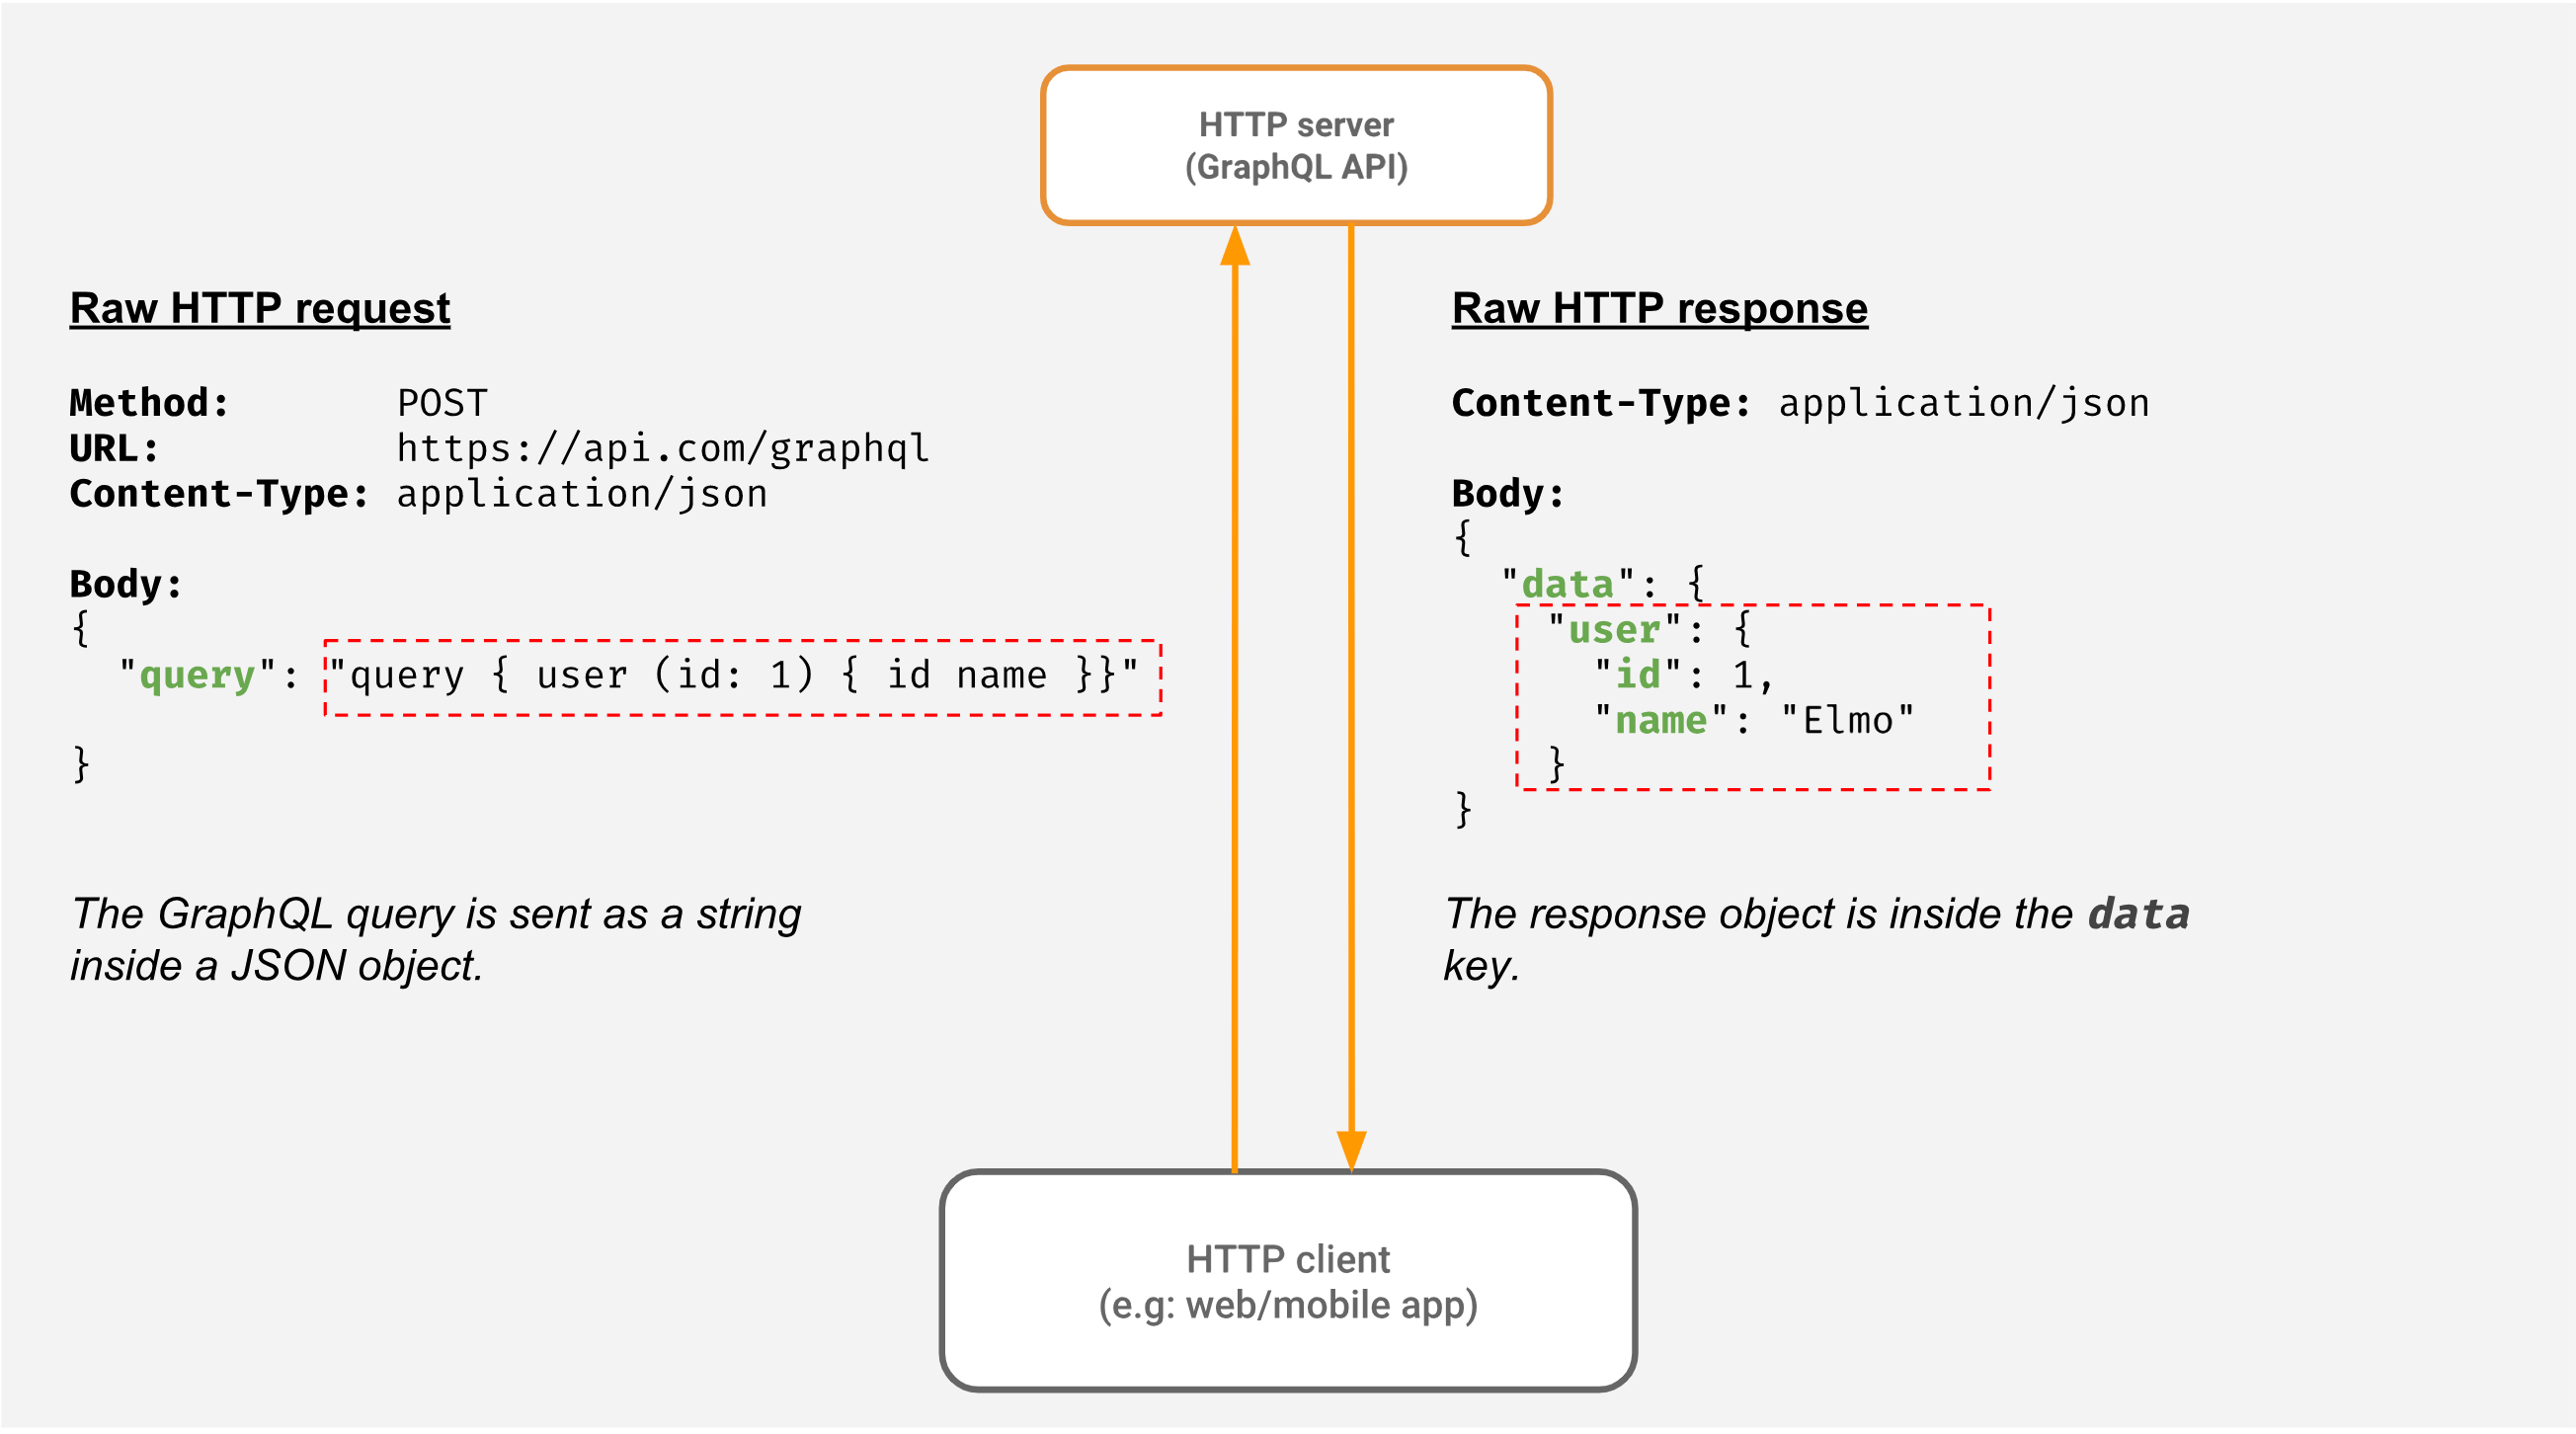
\includegraphics[width=0.9\linewidth]{graphql.png}
		\caption{Estrutura GraphQL}
		\label{fig:graphql_structure}
	\end{figure}

\end{frame}

\begin{frame}
	\frametitle{GraphQL}
	\framesubtitle{Comparação com REST}

	\begin{table}
		\renewcommand{\arraystretch}{1.25} % Ajuste este valor conforme necessário
		\begin{tabular}{|p{0.45\linewidth}|p{0.45\linewidth}|}
			\hline
			\textbf{REST}                                                                 & \textbf{GraphQL}                                                                                \\ \hline
			É uma arquitetura                                                             & É uma linguagem de consulta                                                                     \\ \hline
			Os dados são expostos como recursos                                           & Os dados são expostos como um grafo                                                             \\ \hline
			Overfetching ou underfetching são comuns.                                     & Os clientes solicitam apenas os dados necessários, evitando overfetching e underfetching.       \\ \hline
			Múltiplos endpoints para diferentes recursos.                                 & Um único ponto de entrada para todas as operações.                                              \\ \hline
			Operações de escrita (POST, PUT, DELETE) têm endpoints separados.             & Mutações são tratadas no mesmo sistema de tipos e no mesmo endpoint que as consultas.           \\ \hline
			Utiliza diversos métodos HTTP (GET, POST, PUT, DELETE).                       & Usa o método POST para todas as operações. Pode ser usado com qualquer protocolo de transporte. \\ \hline
			Pode exigir versionamento da API para adicionar ou modificar funcionalidades. & Não requer versionamento devido à flexibilidade nas consultas.                                  \\ \hline
		\end{tabular}
		\caption{REST vs GraphQL}
		\label{tab:rest_graphql}

	\end{table}

\end{frame}

\begin{frame}
	\frametitle{GraphQL}
	\framesubtitle{Mutation}

	\begin{block}{Mutation}
		\begin{itemize}
			\item É um tipo de operação que permite \yellowbox{criar, atualizar ou excluir dados.}
			\item É semelhante a uma operação de escrita no REST.
			\item As mutações são tratadas no mesmo sistema de tipos e no mesmo endpoint que as
			      consultas.
		\end{itemize}
	\end{block}

	\begin{figure}
		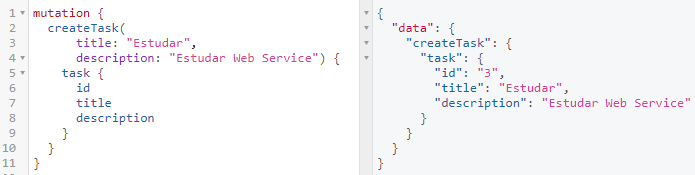
\includegraphics[width=0.9\linewidth]{gql_mutation.png}
		\caption{Exemplo de Mutation}
		\label{fig:graphql_mutation}
	\end{figure}

\end{frame}

\begin{frame}
	\frametitle{GraphQL}
	\framesubtitle{Query}

	\begin{block}{Query}
		\begin{itemize}
			\item É um tipo de operação que permite \yellowbox{recuperar dados.}
			\item É semelhante a uma operação de leitura no REST.
			\item As consultas são tratadas no mesmo sistema de tipos e no mesmo endpoint que as
			      mutações.
		\end{itemize}
	\end{block}

	\begin{figure}
		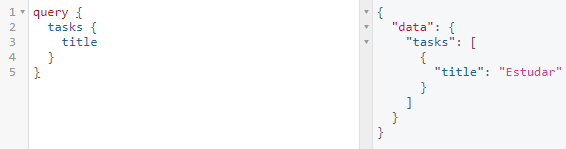
\includegraphics[width=0.9\linewidth]{gql_query.png}
		\caption{Exemplo de Query}
		\label{fig:graphql_query}
	\end{figure}

\end{frame}

\subsection{Experimentos}

\begin{frame}
	\frametitle{GraphQL}
	\framesubtitle{Experimentos}
	{\small
		\begin{block}{Experimento 1}
			\begin{itemize}
				\item Consumir a API GraphQL
				      \href{https://graphqlpokemon.favware.tech/v8}{https://graphqlpokemon.favware.tech/v8}.
				\item Use uma ferramenta como o \href{https://www.thunderclient.com/}{Thunder Client}
				      para testar a API.
				\item Navegue pela documentação da API e teste os endpoints.
			\end{itemize}
		\end{block}

		\begin{block}{Experimento 2}
			Consumir a API GraphQL \href{https://countries.trevorblades.com/}{Countries}. \\
			Repositório da API: \href{https://github.com/trevorblades/countries}{GitHub}.
			\begin{itemize}
				\item Utilizar uma biblioteca/framework de sua escolha para o desenvolvimento
				      frontend (por exemplo, React, Vue, Angular, etc.).
				\item Fazer solicitações HTTP para a API Countries
				      (https://countries.trevorblades.com/) para obter informações sobre os países.
			\end{itemize}
		\end{block}
	}

\end{frame}

\end{document}
